\chapter{Conclusão}\label{sec:conclusion}
Atualmente as empresas, para além de gerirem os seus principais processos de negócio, têm também uma dinâmica significativa de
atividades internas para as ajudar no seu crescimento e competitividade. 
Nem sempre é fácil manter uma boa dinâmica das atividades internas de uma empresa porém, com uma plataforma que permite a gestão das mesmas, torna-se mais simples.
É esse o objetivo do projeto \textit{Collaboration Platform}, no sentido em que promove uma boa gestão destas necessidades e permite que todos os funcionários exponham as suas vontades.
\par
Numa fase inicial do desenvolvimento do projeto, devido à pesquisa e aprendizagem de algumas tecnologias novas, o desenvolvimento ocorreu de forma mais lenta. 
A maior dificuldade encontrada foi a aprendizagem de como desenvolver aplicações numa plataforma nova e desconhecida, com uma utilização crescente no mercado, sendo também diferente do habitual caracterizando-se por um ambiente gráfico de desenvolvimento \textit{low-code}. 
A gestão do progresso do desenvolvimento do projeto foi realizada utilizando uma metodologia de trabalho ágil, o \textit{Scrum~\cite{scrum}}, sendo um aspeto positivo a ser realçado, pois contribuiu para o processo de aprendizagem, uma vez que se trata de uma metodologia muito utilizada no mercado atual.
\par
Após ultrapassados esses obstáculos relacionados com o primeiro contato, o ritmo de trabalho aumentou de forma considerável e foi possível implementar as funcionalidades de forma mais rápida.
Esta boa adaptação ao método de trabalho permitiu que os requisitos propostos fossem cumpridos com sucesso e ainda houvesse tempo para ambicionar atingir outros de caráter 
opcional, nomeadamente a confirmação de presenças através de \textit{QR Code}. 
\par
Ao longo do desenvolvimento da \textit{Collaboration Platform} o grupo deparou-se com diversos obstáculos e decisões de implementação que permitiam boas discussões acerca de como deveríamos proceder.
Um dos principais obstáculos foi o facto da aplicação ser de natureza \textit{reactive}, isto é, passível de ser utilizada tanto em dispositivos móveis (\textit{tablet e telemóvel}) como em \textit{desktop} e o que faz com que o 
seu desenvolvimento tenha um cuidado especial com as diferenças que cada dispositivo apresenta.




\begin{figure}[H]
  \centering 
  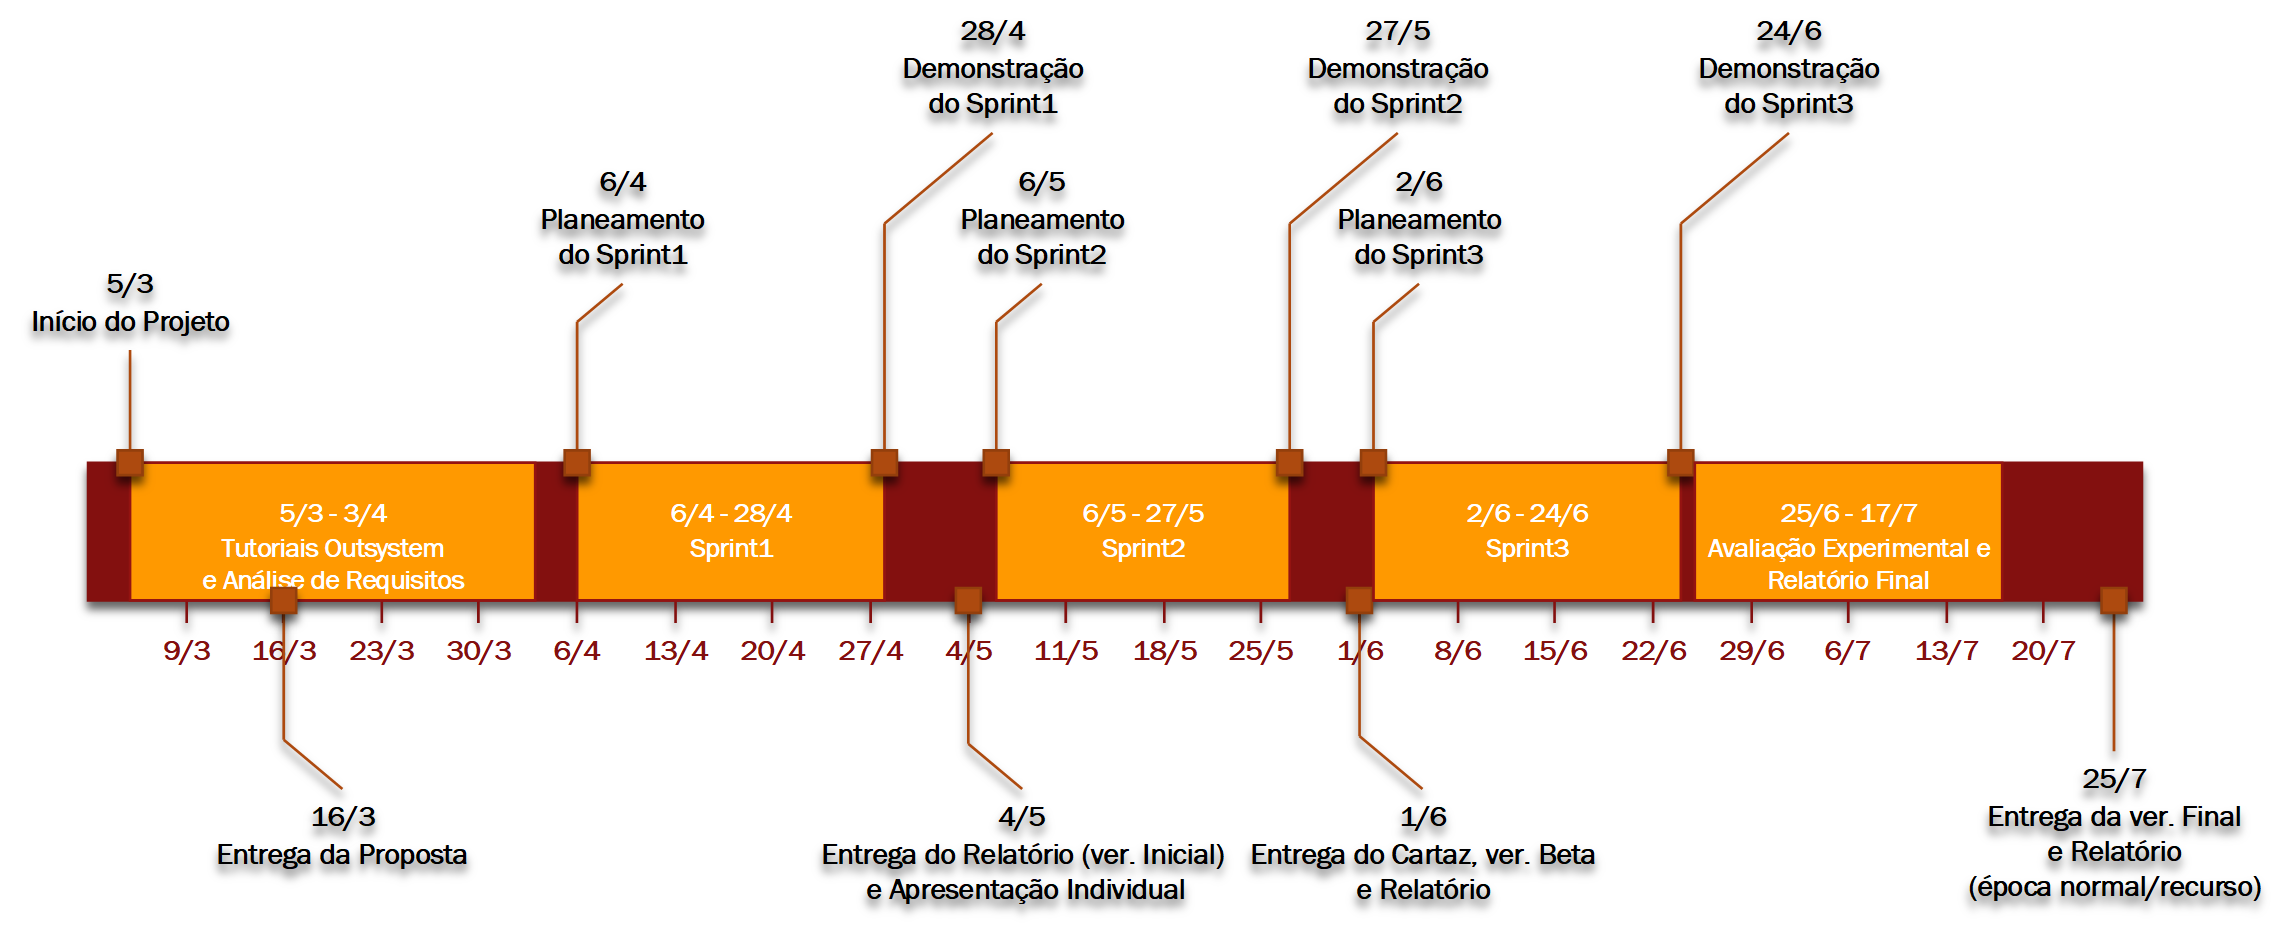
\includegraphics[scale=0.5]{figures/Timeline.png}
  \caption{Timeline}\label{fig:timeline}
\end{figure}